\documentclass[11pt]{article}

% ---------------------------------------------------------------------------
% Panduan Kode: Cross-Layer Grace-Convergence Controller
% Dokumen ini dibangun dengan pdflatex (BUKAN xelatex). Tidak memakai fontspec.
% babel TIDAK dipakai supaya pasti ter-build di mesin mana pun (paket
% babel-bahasa Indonesia belum tentu terpasang). Seluruh ISI berbahasa Indonesia.
% ---------------------------------------------------------------------------

\usepackage[T1]{fontenc}
\usepackage[utf8]{inputenc}
\usepackage{amsmath}
\usepackage[margin=1in]{geometry}
\usepackage{parskip}
\usepackage{xcolor}
\usepackage{graphicx}
\usepackage{booktabs}
\usepackage{enumitem}
\usepackage{longtable}
\usepackage{array}
\usepackage{listings}
\usepackage[colorlinks=true,linkcolor=NavyBlue,urlcolor=NavyBlue,citecolor=NavyBlue]{hyperref}

% Warna -----------------------------------------------------------------------
\definecolor{NavyBlue}{RGB}{31,59,115}
\definecolor{CodeBg}{RGB}{246,247,249}
\definecolor{CodeKw}{RGB}{20,80,160}
\definecolor{CodeStr}{RGB}{40,120,40}
\definecolor{CodeCom}{RGB}{120,120,120}
\definecolor{CodeAtom}{RGB}{150,40,120}
\definecolor{RuleGray}{RGB}{200,200,200}

% Gaya listing umum -----------------------------------------------------------
\lstset{
  basicstyle=\ttfamily\footnotesize,
  backgroundcolor=\color{CodeBg},
  frame=single,
  rulecolor=\color{RuleGray},
  framesep=4pt,
  breaklines=true,
  breakatwhitespace=false,
  postbreak=\mbox{\textcolor{RuleGray}{$\hookrightarrow$}\space},
  columns=fullflexible,
  keepspaces=true,
  showstringspaces=false,
  tabsize=2,
  captionpos=b,
  xleftmargin=10pt,
  xrightmargin=4pt,
  aboveskip=8pt,
  belowskip=8pt,
}

% Definisi bahasa Elixir untuk listings (tidak ada bawaan) ---------------------
\lstdefinelanguage{elixir}{
  morekeywords={def,defp,defmodule,defmacro,defstruct,defdelegate,do,end,fn,case,cond,
    if,else,unless,when,and,or,not,in,for,with,receive,after,try,catch,rescue,raise,
    use,alias,import,require,quote,unquote,true,false,nil,@impl,@moduledoc,@doc,@spec,
    @type,@typedoc},
  otherkeywords={|>,->,<-,=>,::,\&},
  sensitive=true,
  morecomment=[l]{\#},
  morestring=[b]",
  morestring=[b]',
  keywordstyle=\color{CodeKw}\bfseries,
  commentstyle=\color{CodeCom}\itshape,
  stringstyle=\color{CodeStr},
  identifierstyle=\color{black},
}

% Definisi bahasa YAML --------------------------------------------------------
\lstdefinelanguage{yaml}{
  keywords={true,false,null,name,kind,apiVersion,metadata,spec,template,containers,
    image,ports,env,value,replicas,selector,strategy,rollingUpdate,maxUnavailable,
    maxSurge,lifecycle,preStop,exec,command,readinessProbe,livenessProbe,httpGet,
    path,port,namespace,labels,rules,apiGroups,resources,verbs,roleRef,subjects},
  sensitive=true,
  comment=[l]{\#},
  morestring=[b]",
  morestring=[b]',
  keywordstyle=\color{CodeKw}\bfseries,
  commentstyle=\color{CodeCom}\itshape,
  stringstyle=\color{CodeStr},
}

% Alias gaya siap pakai -------------------------------------------------------
\lstdefinestyle{ex}{language=elixir}
\lstdefinestyle{yml}{language=yaml}
\lstdefinestyle{sh}{language=bash,keywordstyle=\color{CodeKw}\bfseries,
  commentstyle=\color{CodeCom}\itshape,stringstyle=\color{CodeStr}}

% Perintah bantu inline -------------------------------------------------------
\newcommand{\code}[1]{\texttt{\small #1}}
\newcommand{\istilah}[1]{\textbf{#1}}

\setlist{topsep=3pt,itemsep=2pt,parsep=0pt}

% =============================================================================
\title{\textbf{Panduan Kode (untuk Mahasiswa)}\\[4pt]
\large Cross-Layer Grace-Convergence Controller:\\
Menyambung Terminasi Pod Kubernetes dengan Konvergensi Cluster Elixir/BEAM}
\author{Dokumentasi teknis proyek \code{01\_cross\_layer\_grace\_controller}}
\date{Dihasilkan otomatis --- versi panduan kode}

% =============================================================================
\begin{document}
\maketitle

\begin{abstract}
\noindent
Dokumen ini menjelaskan \textbf{kode} dari sebuah \emph{controller fault-tolerance lintas-lapis}:
sistem yang membuat Kubernetes dan runtime Elixir/BEAM ``berbicara'' satu sama lain saat sebuah pod
dimatikan. Tujuannya menutup apa yang kami sebut \emph{grace gap}: celah antara waktu tetap yang
diberikan Kubernetes sebelum mematikan paksa sebuah pod, dan waktu yang sebenarnya dibutuhkan runtime
untuk memindahkan (handoff) state in-memory-nya ke node lain. Panduan ini ditulis dengan
\textbf{bahasa yang mudah} untuk mahasiswa S1 tahun ke-3 Teknik Informatika: setiap istilah teknis
dijelaskan saat pertama kali muncul, disertai analogi sehari-hari, cuplikan kode asli, dan
\textbf{langkah persis} untuk menjalankan seluruh eksperimen (RQ1--RQ8). Semua nama fungsi, file, dan
angka diambil langsung dari kode sumber di
\code{01\_cross\_layer\_grace\_controller/}.
\end{abstract}

\tableofcontents
\bigskip
\hrule
\bigskip

% =============================================================================
\section{Pendahuluan: Masalah ``Grace Gap''}
\label{sec:intro}

\subsection{Gambaran singkat}
Bayangkan sebuah aplikasi yang menyimpan banyak data penting \emph{di memori} (RAM), bukan di
database: misalnya ribuan ``ruang chat'', sesi game, atau keranjang belanja yang sedang aktif. Aplikasi
seperti ini dijalankan di atas \istilah{Kubernetes} (sistem yang mengatur banyak container/aplikasi di
banyak mesin) dan ditulis dengan \istilah{Elixir} yang berjalan di atas mesin virtual bernama
\istilah{BEAM} (mesin virtual milik bahasa Erlang/Elixir, terkenal untuk sistem yang harus selalu
hidup).

Masalah muncul ketika Kubernetes perlu mematikan salah satu pod (unit aplikasi terkecil di
Kubernetes), misalnya saat \istilah{rolling update} (memperbarui aplikasi versi-demi-versi tanpa
mematikan semuanya sekaligus). Kalau state di RAM belum sempat dipindahkan ke node lain sebelum pod
dimatikan paksa, \textbf{state itu hilang}. Itulah masalah inti yang ditangani proyek ini.

\subsection{Apa itu terminasi pod Kubernetes?}
Ketika Kubernetes ingin menghentikan sebuah pod, ia tidak langsung ``mencabut steker''. Urutannya:
\begin{enumerate}
  \item Kubernetes mengirim sinyal \code{SIGTERM} ke proses di dalam pod. \istilah{SIGTERM} adalah
  sinyal sistem operasi yang artinya ``tolong berhenti dengan rapi''. Proses \emph{boleh} menanganinya
  dan melakukan pembersihan.
  \item Kubernetes menunggu sejumlah detik tetap, yang disebut \istilah{termination grace period}
  (di manifest Kubernetes namanya \code{terminationGracePeriodSeconds}). Anggap ini ``waktu toleransi''
  yang diberikan untuk berberes.
  \item Setelah waktu itu habis, Kubernetes mengirim \code{SIGKILL}. \istilah{SIGKILL} \textbf{tidak
  bisa} ditangkap atau diabaikan --- proses langsung mati seketika. Apa pun yang belum selesai, hilang.
\end{enumerate}

\paragraph{Analogi.} Bayangkan Anda penyewa kamar kos dan diminta pindah. Pemilik kos berkata:
``Saya beri waktu \emph{tepat 30 menit} untuk mengangkut semua barang; lewat dari itu, semua yang
tersisa saya buang.'' Kalau barang Anda sedikit, 30 menit lebih dari cukup. Tetapi kalau Anda baru
saja belanja banyak (beban tinggi), 30 menit bisa tidak cukup, dan barang sisa terbuang. ``Waktu
toleransi'' (grace period) yang \emph{tetap} itulah sumber masalahnya.

\subsection{Apa itu handoff BEAM?}
Di Elixir/BEAM, satuan kerja terkecil adalah \istilah{proses} (sangat ringan, bukan proses sistem
operasi; satu node BEAM bisa menjalankan jutaan). Setiap proses stateful menyimpan datanya sendiri di
memori. Ketika sebuah node akan pergi, datanya harus dipindahkan ke node yang bertahan. Pemindahan
state dari node yang akan mati ke node lain inilah yang disebut \istilah{handoff}.

Di proyek ini handoff berarti: \emph{baca state proses $\rightarrow$ matikan proses lokal $\rightarrow$
hidupkan kembali proses itu di node ``survivor'' (yang bertahan) dengan state yang sama}. Kalau handoff
belum selesai saat \code{SIGKILL} datang, proses-proses yang belum sempat dipindah (beserta datanya)
lenyap.

\subsection{Mengapa grace period \emph{tetap} itu salah}
Inti masalahnya: berapa detik yang ``cukup'' itu \textbf{bergantung pada beban saat itu}, bukan angka
konstan.
\begin{itemize}
  \item \textbf{Terlalu pendek} (misal tetap 30 detik): saat beban tinggi, handoff terpotong
  \code{SIGKILL}, dan state hilang. Ini pelanggaran \emph{correctness} (kebenaran).
  \item \textbf{Terlalu panjang} (misal tetap 300 detik untuk berjaga-jaga): setiap pod butuh waktu
  lama untuk benar-benar mati, sehingga setiap rolling update jadi sangat lambat. Ini pemborosan
  (\emph{efficiency}).
\end{itemize}
Celah antara grace tetap dan kebutuhan handoff sebenarnya inilah yang disebut \textbf{grace gap}.
Informasi untuk menghitung deadline yang tepat (berapa proses tersisa, secepat apa bisa dipindah) ada
di \emph{runtime} (BEAM), tetapi kontrol yang menegakkan deadline ada di \emph{orkestrator}
(Kubernetes), dan \textbf{tidak ada yang menghubungkan keduanya}. Proyek ini membangun jembatan itu.

\subsection{Apa yang dilakukan controller ini}
\label{sec:grace-formula}
Controller menghitung grace period secara \emph{adaptif} dari sinyal runtime. Kebijakannya:
\[
  g = \mathrm{clamp}\!\left(T_d + \frac{|H|}{\rho} + T_c + \sigma,\; g_{\min},\; g_{\max}\right)
\]
dengan arti tiap simbol:
\begin{itemize}
  \item $|H|$ = \textbf{backlog handoff}: berapa proses stateful yang masih harus dipindahkan.
  \item $\rho$ (dibaca ``rho'') = \textbf{laju handoff}: berapa proses per detik yang bisa dipindahkan.
  \item $T_c$ = \textbf{waktu konvergensi}: waktu agar cluster ``tenang'' kembali (membership stabil,
  registry sinkron) setelah node pergi.
  \item $T_d$ = \textbf{waktu drain}: waktu menyelesaikan permintaan yang sedang berjalan sebelum
  state dipindahkan.
  \item $\sigma$ (dibaca ``sigma'') = \textbf{margin keamanan}: bumper tambahan agar tidak pas di tepi.
  \item $g_{\min}, g_{\max}$ = batas bawah dan atas, supaya grace tidak terlalu kecil maupun terlalu
  besar.
\end{itemize}
Suku kunci $|H|/\rho$ secara intuitif adalah ``jumlah pekerjaan / kecepatan = waktu'', yaitu perkiraan
lama handoff. \textbf{Invariant keselamatan} (aturan yang harus selalu benar agar tidak ada state
hilang):
\[
  g \;\ge\; T_d + \frac{|H|}{\rho} + T_c .
\]
Selama grace yang diberikan tidak lebih kecil dari kebutuhan sebenarnya, handoff tidak akan terpotong.

\paragraph{Analogi.} Kembali ke kasus pindah kos: controller ini seperti seorang asisten cerdas yang
melihat berapa banyak barang Anda sekarang ($|H|$), seberapa cepat tukang angkut bekerja ($\rho$),
lalu berkata kepada pemilik kos: ``Beri dia tepat $|H|/\rho$ menit, ditambah sedikit bumper.'' Tidak
terlalu mepet (barang aman) dan tidak terlalu lama (kamar cepat kosong).

% =============================================================================
\section{Struktur Folder Proyek}
\label{sec:struktur}

Proyek tinggal di \code{01\_cross\_layer\_grace\_controller/}. Dokumen yang sedang Anda baca berada di
folder baru \code{code\_guide/}, sejajar dengan \code{code/} dan \code{paper/}. Berikut pohon
direktori inti (folder hasil build seperti \code{\_build/} dan \code{deps/} dihilangkan):

\begin{lstlisting}[basicstyle=\ttfamily\scriptsize]
01_cross_layer_grace_controller/
|-- README.md            # status proyek + cara build (baca paling awal)
|-- CONTEXT.md           # catatan konvensi (jangan diregres)
|-- OUTLINE.md           # kerangka paper
|-- code/                # ARTIFACT + harness eksperimen
|   |-- README.md
|   |-- DESIGN.md        # analisis -> requirement -> desain -> validasi
|   |-- Dockerfile       # 1 image; GRACE_ROLE memilih app vs operator
|   |-- app/             # proyek Elixir/OTP `grace_convergence`
|   |   |-- README.md
|   |   |-- mix.exs      # daftar dependency + metadata proyek
|   |   |-- mix.lock     # versi dependency yang dikunci
|   |   |-- config/      # config.exs, dev.exs, test.exs, prod.exs
|   |   |-- lib/
|   |   |   |-- grace_convergence.ex          # modul puncak (delegasi)
|   |   |   `-- grace_convergence/            # semua modul inti
|   |   |       |-- application.ex            # pohon supervisi (boot)
|   |   |       |-- grace.ex                  # kebijakan grace = clamp(...)
|   |   |       |-- probe.ex                  # sensor konvergensi (EWMA)
|   |   |       |-- stateful_worker.ex        # 1 proses stateful
|   |   |       |-- workers.ex                # buat/hitung/cari worker
|   |   |       |-- handoff.ex                # pindahkan state ke survivor
|   |   |       |-- shutdown.ex               # hook terminasi adaptif
|   |   |       |-- probe_http.ex             # /probe /healthz /drain
|   |   |       |-- operator.ex               # operator Kubernetes (kubectl)
|   |   |       |-- presence.ex               # Phoenix.Tracker (RQ8)
|   |   |       `-- harness.ex                # driver eksperimen
|   |   |-- harness/      # skrip .exs untuk menjalankan eksperimen
|   |   |   |-- run.exs        # tabel 2-beban (RQ1/RQ2)
|   |   |   |-- sweep.exs      # sweep + rollout + overhead + sensitivitas
|   |   |   |-- repeats.exs    # pengulangan N=10 / N=5 (confidence interval)
|   |   |   |-- scale.exs      # |H| 1k..40k (RQ6)
|   |   |   `-- presence.exs   # konvergensi Phoenix.Presence (RQ8)
|   |   |-- scripts/
|   |   |   `-- cluster_probe.exs  # menonton handoff 2-node secara manual
|   |   `-- test/
|   |       |-- grace_test.exs           # 6 unit test untuk Grace
|   |       `-- cluster_handoff_test.exs # 2 test integrasi cluster
|   |-- k8s/             # manifest + skrip Kubernetes
|   |   |-- rbac.yaml         # izin (ServiceAccount + Role)
|   |   |-- app.yaml          # Deployment app + Service + PDB + preStop
|   |   |-- operator.yaml     # Deployment operator
|   |   |-- netem.sh          # injeksi latensi nyata tc netem (RQ7)
|   |   `-- faults.sh         # injeksi fault (fail-safe)
|   `-- analysis/
|       `-- plot.py          # data/*.csv -> figures/*.pdf (matplotlib)
|-- data/                # hasil eksperimen (CSV; hanya data nyata)
|-- figures/             # diagram (.puml/.dot) + plot (.pdf)
|-- paper/               # manuskrip LaTeX (main.tex, references.bib, ...)
|-- code_guide/          # << dokumen INI (panduan kode)
|-- cover_letter/        # surat pengantar submisi
`-- declarations/        # deklarasi (etika, dsb.)
\end{lstlisting}

Tabel berikut merangkum \textbf{tanggung jawab} tiap folder dan file penting.

\begin{longtable}{@{}p{0.34\linewidth} p{0.60\linewidth}@{}}
\toprule
\textbf{Path} & \textbf{Tanggung jawab} \\
\midrule
\endhead
\code{README.md} (top) & Ringkasan status proyek, keputusan desain, cara build. Baca paling awal. \\
\code{CONTEXT.md} & Catatan konvensi penulisan \& gotcha eksperimen yang tidak boleh diregres. \\
\code{code/DESIGN.md} & Alur analisis $\rightarrow$ requirement (FR/NFR) $\rightarrow$ desain $\rightarrow$ rencana validasi (V1--V7). \\
\code{code/app/} & Proyek Elixir/OTP \code{grace\_convergence}: seluruh logika inti. \\
\code{code/app/mix.exs} & Definisi proyek + daftar dependency (Horde, libcluster, Bandit, Plug, Jason, phoenix\_pubsub). \\
\code{code/app/config/} & Konfigurasi per-lingkungan: \code{config.exs} (umum), \code{test.exs}, \code{prod.exs} (strategi libcluster Kubernetes). \\
\code{code/app/lib/grace\_convergence/} & 11 modul inti (grace, probe, worker, handoff, shutdown, operator, dll.). Dirinci di Bagian~\ref{sec:modul}. \\
\code{code/app/harness/} & Skrip \code{.exs} yang \emph{menjalankan} eksperimen dan menulis CSV ke \code{data/}. \\
\code{code/app/scripts/cluster\_probe.exs} & Alat manual untuk menonton satu handoff 2-node secara langsung. \\
\code{code/app/test/} & \code{grace\_test.exs} (6 unit test kebijakan grace) dan \code{cluster\_handoff\_test.exs} (2 test integrasi cluster nyata). \\
\code{code/k8s/} & Manifest Kubernetes (\code{rbac.yaml}, \code{app.yaml}, \code{operator.yaml}) + skrip \code{netem.sh} \& \code{faults.sh}. \\
\code{code/analysis/plot.py} & Mengubah \code{data/*.csv} menjadi \code{figures/*.pdf} memakai matplotlib. \\
\code{code/Dockerfile} & Satu image multi-stage; variabel \code{GRACE\_ROLE} memilih peran \code{app} atau \code{operator}. \\
\code{data/} & Berkas CSV hasil eksperimen --- \emph{hanya data nyata}, tidak ada angka fiktif. \\
\code{figures/} & Sumber diagram (\code{.puml}/\code{.dot}) dan plot hasil (\code{.pdf}). \\
\code{paper/} & Manuskrip LaTeX (memakai kelas Wiley; bukan dokumen ini). \\
\code{code\_guide/} & Dokumen panduan kode ini (kelas \code{article} standar). \\
\bottomrule
\end{longtable}

% =============================================================================
\section{Library yang Dipakai dan Perannya}
\label{sec:library}

Sebelum masuk ke tabel, beberapa istilah dasar yang sering muncul:

\begin{description}[leftmargin=1.4em,style=nextline]
  \item[GenServer] ``Server process'' standar di OTP (kerangka kerja Erlang/Elixir untuk sistem
  tahan-gagal). Sebuah GenServer memiliki state privat dan menangani pesan \emph{satu per satu}.
  Caller bicara via \code{GenServer.call} (sinkron: menunggu balasan) atau \code{GenServer.cast}
  (asinkron: kirim lalu lupakan). Banyak modul di proyek ini adalah GenServer.
  \item[Supervisor] Proses ``pengawas'' yang menjalankan proses-proses lain (anak) dan
  me-\emph{restart} mereka bila mati. Filosofi Erlang: ``let it crash'' --- biarkan proses mati, lalu
  supervisor menghidupkannya lagi ke kondisi bersih. \istilah{DynamicSupervisor} adalah supervisor
  yang anaknya dibuat sesuai kebutuhan saat runtime (bukan daftar tetap saat boot).
  \item[CRDT] \emph{Conflict-free Replicated Data Type} --- struktur data yang bisa diubah secara
  lokal di banyak node, lalu otomatis ``menyatu'' (merge) ke hasil yang sama di semua node tanpa perlu
  koordinasi pusat. Cocok untuk sistem terdistribusi. Horde memakai CRDT.
  \item[Operator] Pola di Kubernetes: sebuah program yang terus ``mengawasi'' kondisi cluster dan
  ``mendamaikan'' (reconcile) kondisi nyata ke kondisi yang diinginkan. Operator di proyek ini membaca
  probe tiap pod lalu menambal \code{terminationGracePeriodSeconds}.
\end{description}

\begin{longtable}{@{}p{0.20\linewidth} p{0.74\linewidth}@{}}
\toprule
\textbf{Library / Tool} & \textbf{Peran dalam proyek} \\
\midrule
\endhead
\textbf{Elixir / OTP} & Bahasa dan platform dasar. Menyediakan \code{GenServer} (Probe, Shutdown,
StatefulWorker, Operator, Presence), \code{Supervisor} \& \code{DynamicSupervisor}
(\code{WorkerSup} menjadi tuan rumah worker), serta \code{Application} (boot pohon supervisi). \\
\textbf{Horde} (\code{\~{} 0.9}) & Registry terdistribusi berbasis delta-CRDT + dukungan handoff.
\code{Horde.Registry} memberi tiap worker \emph{identitas unik se-cluster} sehingga node mana pun bisa
mencari worker berdasarkan kunci, walau worker pindah node. \\
\textbf{libcluster} (\code{\~{} 3.3}) & Membentuk cluster BEAM secara otomatis. Lokal memakai strategi
\code{Gossip}; di Kubernetes memakai \code{Cluster.Strategy.Kubernetes} (menemukan pod via headless
service). Lihat \code{config/prod.exs}. \\
\textbf{Bandit} (\code{\~{} 1.5}) & Web server untuk menyajikan endpoint HTTP probe (\code{/probe},
\code{/healthz}, \code{/drain}). Dijalankan dari pohon supervisi di \code{application.ex}. \\
\textbf{Plug} (\code{\~{} 1.16}) & Lapisan ``router'' HTTP. \code{GraceConvergence.ProbeHTTP} memakai
\code{Plug.Router} untuk memetakan path ke handler. \\
\textbf{Jason} (\code{\~{} 1.4}) & Encode/decode JSON. Probe membalas dalam JSON; operator mem-parsing
JSON pod \& probe, dan menyusun patch JSON untuk \code{kubectl}. \\
\textbf{phoenix\_pubsub} (\code{\~{} 2.1}) & Menyediakan \code{Phoenix.PubSub} dan
\code{Phoenix.Tracker} --- mesin CRDT di balik \code{Phoenix.Presence}. Dipakai sebagai
\emph{workload realistis} untuk mengukur waktu konvergensi nyata $T_c$ (RQ8). \\
\textbf{kubectl via \code{System.cmd}} & Operator memanggil biner \code{kubectl} dari Elixir
(\code{System.cmd/2}) untuk mendaftar pod dan menambal Deployment. Jadi operator ini adalah
\emph{GenServer biasa yang memanggil \code{kubectl}} --- \textbf{bukan} framework Bonny. \\
\textbf{kind} & ``Kubernetes IN Docker'' --- menjalankan cluster Kubernetes di dalam container Docker
di satu mesin. Dipakai untuk eksperimen V3 dan RQ7. \\
\textbf{kubectl} & CLI Kubernetes untuk apply manifest, melihat log, scale, dsb. \\
\textbf{docker} & Membangun image aplikasi dan menjalankan node kind. \\
\textbf{Graphviz} (\code{dot}) & Mesin tata-letak grafik; dipakai PlantUML untuk merender diagram dan
oleh berkas \code{.dot}. \\
\textbf{matplotlib} & Library Python untuk membuat plot; \code{analysis/plot.py} memakainya untuk
membuat seluruh figur \code{eval\_*.pdf}. \\
\textbf{tc / netem} & \code{tc} (traffic control) + modul \code{netem} milik kernel Linux untuk
menyuntikkan latensi jaringan buatan. Dipakai \code{k8s/netem.sh} untuk RQ7. \\
\bottomrule
\end{longtable}

% =============================================================================
\section{Penjelasan Modul-per-Modul}
\label{sec:modul}

Semua modul inti ada di \code{code/app/lib/grace\_convergence/}. Untuk tiap modul: tugas satu kalimat,
fungsi-fungsi kunci, posisinya dalam keseluruhan, dan cuplikan kode \emph{asli} yang pendek.

Sebelum masuk ke detail tiap modul, Gambar~\ref{fig:seq-modules} memberi gambaran besar
\emph{bagaimana modul-modul ini saling memanggil} ketika \emph{satu drain} berlangsung---yakni satu
kali proses pengosongan/evakuasi sebuah node yang akan pergi, di mana semua proses stateful-nya
di-handoff ke node yang bertahan (lihat Glosarium). Bacalah
dari atas ke bawah mengikuti waktu: \code{Shutdown} meminta angka ke \code{Probe}, menghitung grace
lewat \code{Grace}, lalu menyuruh \code{Handoff} memindahkan worker melalui \code{Workers}.

\begin{figure}[ht]
  \centering
  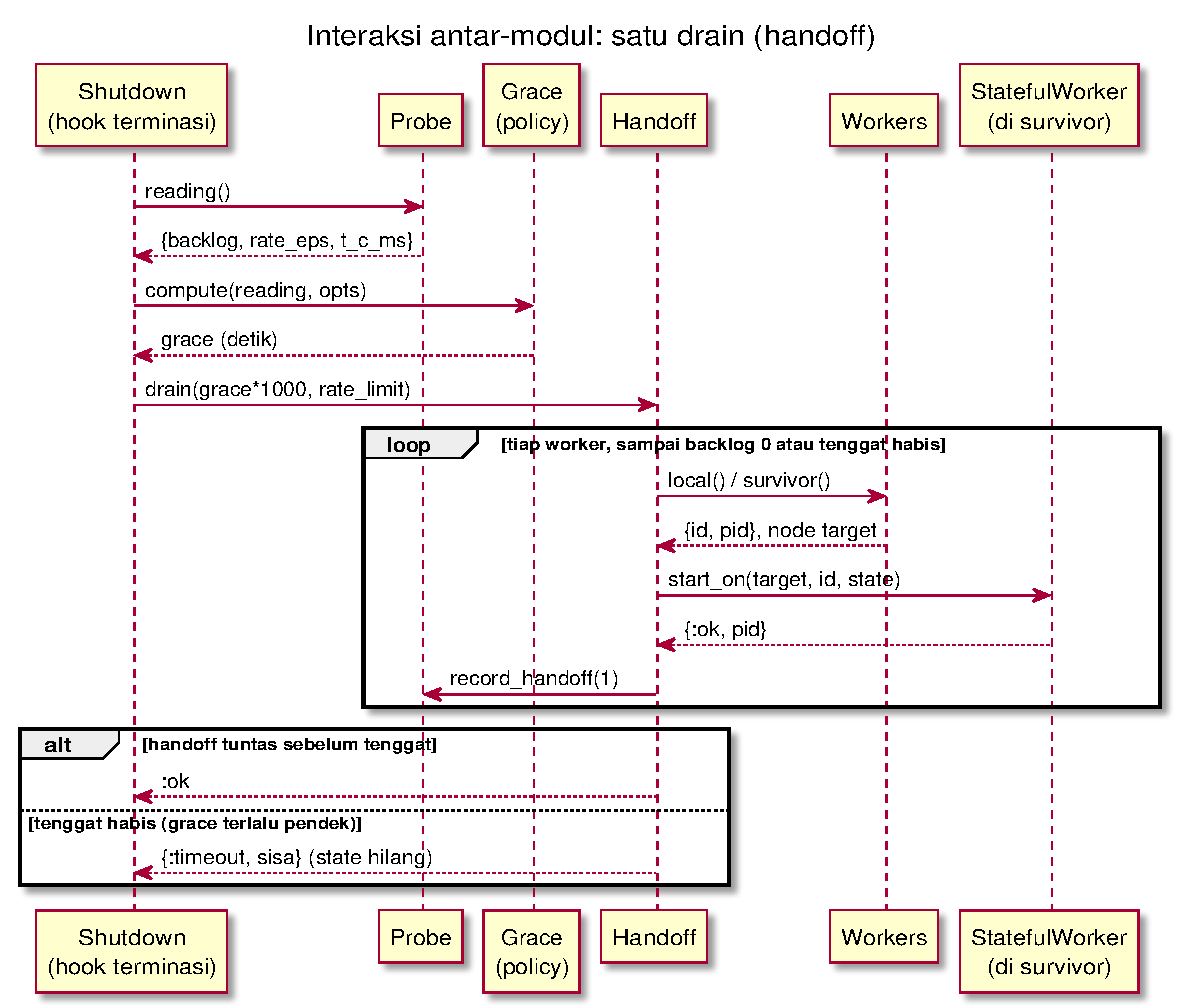
\includegraphics[width=0.92\linewidth]{fig/seq_modules.pdf}
  \caption{\emph{Sequence diagram} (UML) interaksi antar-modul Elixir saat satu drain. Panah padat =
  panggilan; panah putus-putus = balasan. Blok \texttt{loop} menangani satu worker per putaran sampai
  backlog habis atau tenggat (grace) tercapai; blok \texttt{alt} menunjukkan dua akhir yang mungkin:
  \code{:ok} (handoff tuntas) atau \code{\{:timeout, sisa\}} (grace terlalu pendek $\rightarrow$ state
  hilang).}
  \label{fig:seq-modules}
\end{figure}

\subsection{\texttt{GraceConvergence} --- modul puncak}
\textbf{Tugas:} pintu masuk ringkas; hanya mendelegasikan tiga fungsi populer ke modul yang
sebenarnya. \\
\textbf{Posisi:} memudahkan dipakai dari REPL (\code{iex}).
\begin{lstlisting}[style=ex]
defdelegate reading(), to: GraceConvergence.Probe
defdelegate drain_and_await(), to: GraceConvergence.Shutdown
defdelegate start_many(n), to: GraceConvergence.Workers
\end{lstlisting}
\code{defdelegate} berarti ``panggilan ke fungsi ini sebenarnya diteruskan ke modul lain''. Jadi
\code{GraceConvergence.reading()} sama dengan \code{GraceConvergence.Probe.reading()}.

\subsection{\texttt{GraceConvergence.Application} --- pohon supervisi}
\textbf{Tugas:} menentukan proses apa saja yang dijalankan saat aplikasi boot, sesuai \emph{peran}
(\code{app} atau \code{operator}). \\
\textbf{Posisi:} ``akar'' dari segalanya; tanpa modul ini tidak ada yang hidup. \\
\textbf{Fungsi kunci:} \code{start/2} (callback OTP), \code{role/0} (membaca \code{GRACE\_ROLE}).
\begin{lstlisting}[style=ex]
children =
  case role() do
    :operator ->
      [GraceConvergence.Operator]            # pod operator: hanya koordinator

    :app ->
      cluster_children(cfg) ++               # libcluster (pembentuk cluster)
        [
          {Horde.Registry, [name: GraceConvergence.Registry, keys: :unique, members: :auto]},
          {DynamicSupervisor, name: GraceConvergence.WorkerSup, strategy: :one_for_one},
          {Phoenix.PubSub, name: GraceConvergence.PubSub},
          GraceConvergence.Presence,
          GraceConvergence.Probe,
          Supervisor.child_spec({GraceConvergence.Shutdown, []}, shutdown: 310_000)
        ] ++ http_children(cfg)
  end
\end{lstlisting}
Perhatikan \code{shutdown: 310\_000}: supervisor memberi modul \code{Shutdown} hingga 310 detik untuk
menyelesaikan drain saat aplikasi dihentikan secara rapi --- cukup besar agar drain adaptif sempat
berjalan. \code{members: :auto} membuat \code{Horde.Registry} otomatis menemukan node lain.

\subsection{\texttt{GraceConvergence.Grace} --- kebijakan grace}
\textbf{Tugas:} menghitung berapa \emph{detik bulat} grace yang harus diberikan, dari satu pembacaan
probe. \\
\textbf{Posisi:} otak matematis controller (rumus utama; lihat Bagian~\ref{sec:grace-formula}). \\
\textbf{Fungsi kunci:} \code{compute/2} (publik), \code{handoff\_seconds/1} dan \code{t\_c\_seconds/1}
(privat).
\begin{lstlisting}[style=ex]
def compute(reading, opts \\ []) do
  g_min = Keyword.get(opts, :g_min, 5)
  g_max = Keyword.get(opts, :g_max, 120)
  sigma = Keyword.get(opts, :sigma, 5)
  t_d = Keyword.get(opts, :t_d, 1)
  fallback = Keyword.get(opts, :fallback, g_max)

  g =
    case handoff_seconds(reading) do
      :unknown -> fallback                              # tak bisa hitung -> aman: pakai fallback besar
      secs -> t_d + secs + t_c_seconds(reading) + sigma # estimasi: T_d + |H|/rho + T_c + sigma
    end

  g |> max(g_min) |> min(g_max) |> round()             # clamp ke [g_min, g_max], bulatkan
end
\end{lstlisting}
Fungsi \code{handoff\_seconds/1} menghitung $|H|/\rho$ memakai \emph{pattern matching} (mencocokkan
bentuk data). Urutan klausa penting karena Elixir mencoba dari atas ke bawah:
\begin{lstlisting}[style=ex]
# Kasus normal: backlog b dan laju r > 0 -> waktu = pekerjaan / kecepatan = b / r
defp handoff_seconds(%{backlog: b, rate_eps: r})
     when is_number(b) and is_number(r) and r > 0,
     do: b / r

# Tidak ada yang perlu dipindah (backlog 0) -> handoff butuh 0 detik
defp handoff_seconds(%{backlog: 0}), do: 0

# Selain itu (mis. backlog > 0 tapi laju 0/hilang): tak bisa hitung -> :unknown
defp handoff_seconds(_), do: :unknown
\end{lstlisting}
Filosofi penting: bila tidak bisa mengestimasi, jangan menebak --- kembalikan \emph{fallback} yang
besar (\code{:default-safe, never default-fast}). Lebih baik membuang beberapa detik daripada
kehilangan state yang tidak bisa dikembalikan. Perilaku ini diuji di \code{grace\_test.exs} (lihat
Bagian~\ref{sec:tests}).

\subsection{\texttt{GraceConvergence.Probe} --- sensor konvergensi}
\textbf{Tugas:} GenServer read-only yang melaporkan angka runtime yang dibutuhkan kebijakan grace
(terutama laju handoff $\rho$). \\
\textbf{Posisi:} sumber data untuk \code{Grace.compute/2} dan untuk endpoint \code{/probe}. \\
\textbf{Fungsi kunci:} \code{reading/0}, \code{record\_handoff/1}, \code{mark\_drain\_start/0},
\code{reset/0}.

Probe memperkirakan $\rho$ memakai \istilah{EWMA} (\emph{Exponentially Weighted Moving Average}) ---
rata-rata berjalan yang memberi bobot lebih besar pada sampel terbaru, sehingga macet sesaat tidak
merusak estimasi secara permanen. Rumusnya \code{rata\_baru = alpha*sampel + (1-alpha)*rata\_lama},
dengan \code{@alpha = 0.3}:
\begin{lstlisting}[style=ex]
def handle_cast({:handoff, n, ts}, s) do
  rate =
    case s.last_ts do
      nil -> s.rate_eps                                # handoff pertama: belum ada selang waktu
      prev when ts > prev ->
        @alpha * (n * 1000 / (ts - prev)) + (1 - @alpha) * s.rate_eps  # EWMA
      _ -> s.rate_eps                                  # dua event di milidetik sama: hindari bagi 0
    end
  {:noreply, %{s | rate_eps: rate, last_ts: ts, handed: s.handed + n}}
end
\end{lstlisting}
Saat membangun pembacaan, backlog diambil dari \code{Workers.local\_count()} (berapa worker masih di
node ini), dan bila belum ada laju terukur, dipakai laju konfigurasi (\code{:handoff\_rate\_limit}):
\begin{lstlisting}[style=ex]
defp build_reading(s) do
  backlog = Workers.local_count()
  rate = if s.rate_eps > 0, do: s.rate_eps, else: configured_rate()
  %{
    node: Node.self(), backlog: backlog, rate_eps: Float.round(rate, 3),
    t_c_ms: convergence_ms(), in_flight: backlog,
    converged?: Node.list() != [] or backlog == 0, handed_off: s.handed
  }
end
\end{lstlisting}
Catatan: \code{convergence\_ms/0} kini hanya perkiraan kasar (\code{length(Node.list()) * 50}, yakni
$\sim$50 ms per peer). Di produksi sebaiknya diganti sinyal konvergensi terukur --- RQ8 mengukur nilai
$T_c$ nyata memakai Phoenix.Presence dan menunjukkan estimasi 50 ms ini jauh lebih kecil dari kenyataan
($\sim$1{,}5 s), tetapi tertutup oleh margin $\sigma$.

\subsection{\texttt{GraceConvergence.StatefulWorker} --- satu proses stateful}
\textbf{Tugas:} unit kerja yang dilindungi sistem --- objek kecil di memori yang \emph{tidak boleh
hilang} saat node mati. \\
\textbf{Posisi:} ``barang'' yang di-handoff. \\
\textbf{Fungsi kunci:} \code{child\_spec/1}, \code{start\_link/1}, \code{via/1}, \code{state/1},
\code{touch/1}.
\begin{lstlisting}[style=ex]
use GenServer, restart: :transient   # hanya di-restart bila crash; stop sengaja (handoff) dibiarkan

def via(id), do: {:via, Horde.Registry, {@registry, id}}  # alamat lewat registry, bukan PID mentah

def init(opts) do
  id = Keyword.fetch!(opts, :id)
  data = Keyword.get(opts, :state) || %{id: id, updates: 0, born: System.os_time(:millisecond)}
  {:ok, data}                          # pakai state hasil handoff bila ada; jika tidak, buat baru
end
\end{lstlisting}
\code{restart: :transient} penting: handoff mematikan worker dengan \emph{normal} (sengaja), sehingga
supervisor tidak menghidupkannya kembali di node lama --- persis yang kita inginkan. \code{via/1}
membuat \emph{via-tuple}: alamat berbasis kunci di \code{Horde.Registry}, sehingga tetap valid walau
worker pindah node.

\subsection{\texttt{GraceConvergence.Workers} --- buat, hitung, cari worker}
\textbf{Tugas:} kumpulan helper untuk membuat banyak worker, menghitungnya, dan menemukan yang lokal. \\
\textbf{Posisi:} jembatan antara identitas (Horde) dan hosting (DynamicSupervisor lokal). \\
\textbf{Fungsi kunci:} \code{start\_local/2}, \code{start\_on/3}, \code{start\_many/2},
\code{start\_many\_local/2}, \code{stop\_all/0}, \code{all/0}, \code{local/0}, \code{local\_count/0},
\code{survivor/0}.

Keputusan desain penting ada di sini: \emph{identitas} dari \code{Horde.Registry} (unik se-cluster),
tetapi \emph{hosting} dari \code{DynamicSupervisor} lokal --- \textbf{bukan} supervisor terdistribusi
Horde. Alasannya, bila Horde yang menjadi tuan rumah, ia bisa menempatkan ulang worker di node yang
\emph{justru sedang kita kosongkan}. Dengan hosting lokal, controller-lah yang memilih node tujuan saat
handoff.
\begin{lstlisting}[style=ex]
def start_on(node, id, state \\ nil) do
  :rpc.call(node, __MODULE__, :start_local, [id, state])  # jalankan start_local di node lain
end

def local do  # pasangan {key, pid} yang hosted DI node ini DAN masih hidup
  Enum.filter(all(), fn {_key, pid} -> node(pid) == Node.self() and Process.alive?(pid) end)
end

def survivor do                # pilih satu peer yang bertahan, acak; nil bila terisolasi
  case Node.list() do
    [] -> nil
    nodes -> Enum.random(nodes)
  end
end
\end{lstlisting}
Cek \code{Process.alive?/1} di \code{local/0} penting karena \emph{timing} CRDT: saat worker mati,
entri registry-nya masih ``tertinggal'' sesaat sampai penghapusan menyebar ke semua node; tanpa cek
ini, loop drain bisa terus menemukan entri mati dan berputar selamanya. \code{:rpc.call/4} adalah
\istilah{RPC} (\emph{Remote Procedure Call}): menjalankan fungsi di node lain dan mengembalikan
hasilnya.

\subsection{\texttt{GraceConvergence.Handoff} --- pemindah state}
\textbf{Tugas:} mengosongkan worker lokal dengan memindahkan state tiap worker ke node survivor,
di-throttle ke laju tertentu; berhenti saat backlog 0 \emph{atau} deadline habis. \\
\textbf{Posisi:} ``tukang angkut'' yang melaksanakan handoff sebenarnya. Deadline habis sebelum backlog
0 = handoff terpotong = kasus state hilang (RQ1). \\
\textbf{Fungsi kunci:} \code{drain/2}, \code{loop/2} (privat), \code{handoff\_one/2} (privat),
\code{place/4} (privat).
\begin{lstlisting}[style=ex]
def drain(deadline_ms, rate_limit \\ nil) do
  Probe.mark_drain_start()
  loop(now_ms() + deadline_ms, rate_limit)
end

defp loop(deadline, rate_limit) do
  cond do
    Workers.local_count() == 0 -> :ok                         # selesai: semua sudah pindah
    now_ms() >= deadline -> {:timeout, Workers.local_count()} # waktu habis: sisa = yang hilang
    true ->
      case Workers.local() do
        [{id, pid} | _] ->
          case handoff_one(id, pid) do
            :ok -> if rate_limit, do: Process.sleep(max(1, trunc(1000 / rate_limit)))
            :no_survivor -> Process.sleep(100)
          end
          loop(deadline, rate_limit)
        [] -> :ok
      end
  end
end
\end{lstlisting}
Nilai kembalian \code{\{:timeout, remaining\}} adalah inti pembuktian RQ1: \code{remaining} adalah
jumlah worker yang \emph{tidak sempat} dipindah --- inilah ``state hilang''. Pemindahan satu worker:
\begin{lstlisting}[style=ex]
defp handoff_one(id, pid) do
  case Workers.survivor() do
    nil -> :no_survivor
    target ->
      state = safe_state(pid)                       # 1. baca state worker
      _ = DynamicSupervisor.terminate_child(@sup, pid)  # 2. matikan worker lokal
      place(id, state, target, 40)                  # 3. hidupkan di survivor (retry s/d 40x)
      :ok
  end
end
\end{lstlisting}
\code{place/4} mencoba ulang penempatan karena registrasi lama worker yang baru mati bisa membuat Horde
sementara menolak start baru dengan \code{\{:already\_started, dead\_pid\}}; kode menunggu CRDT
membersihkannya lalu mencoba lagi. Setiap penempatan sukses memanggil \code{Probe.record\_handoff(1)}
agar EWMA laju ter-update.

\subsection{\texttt{GraceConvergence.Shutdown} --- hook terminasi adaptif}
\textbf{Tugas:} saat shutdown rapi (atau panggilan eksplisit), menghitung jendela grace sesuai
\emph{policy} terkonfigurasi, lalu menjalankan drain dalam jendela itu. \\
\textbf{Posisi:} penghubung kebijakan (\code{Grace}) dengan eksekusi (\code{Handoff}); inilah yang
dijalankan jalur \code{SIGTERM} (lewat \code{/drain}). \\
\textbf{Fungsi kunci:} \code{drain\_and\_await/0}, \code{terminate/2} (callback), \code{do\_drain/0}
(privat), \code{grace\_for/4} (privat).
\begin{lstlisting}[style=ex]
def init(_) do
  Process.flag(:trap_exit, true)   # tangkap sinyal exit supaya terminate/2 dipanggil saat stop
  {:ok, %{}}
end

def terminate(_reason, _s) do
  do_drain()                       # saat aplikasi dihentikan rapi: jalankan drain dulu
  :ok
end

defp grace_for(:m3, reading, cfg, g_max) do            # policy adaptif: pakai Grace.compute
  Grace.compute(reading, sigma: ..., g_min: ..., g_max: g_max, t_d: ..., fallback: g_max)
end
defp grace_for(:prestop_sleep, _r, cfg, _), do: Keyword.get(cfg, :static_grace, 30)
defp grace_for(:static30, _r, _cfg, _), do: 30
defp grace_for(:static300, _r, _cfg, _), do: 300
\end{lstlisting}
Empat policy itu (FR6) memungkinkan harness membandingkan controller adaptif (\code{:m3}) dengan tiga
baseline tetap. Hasil drain dilaporkan sebagai map \code{\%\{policy, grace\_s, result, lost\}}, dengan
\code{lost} dihitung dari \code{\{:timeout, remaining\}}.

\subsection{\texttt{GraceConvergence.ProbeHTTP} --- endpoint HTTP}
\textbf{Tugas:} menyediakan tiga endpoint HTTP yang dipakai operator dan hook \code{preStop}. \\
\textbf{Posisi:} permukaan jaringan dari node app. \\
\textbf{Fungsi kunci:} rute \code{GET /probe}, \code{GET /healthz}, \code{POST /drain}.
\begin{lstlisting}[style=ex]
get "/probe" do                                   # operator membaca ini untuk menghitung grace
  send_resp(conn, 200, Jason.encode!(Probe.reading()))
end
get "/healthz", do: send_resp(conn, 200, "ok")    # liveness/readiness probe Kubernetes
post "/drain" do                                  # dipanggil hook preStop saat SIGTERM
  result = Shutdown.drain_and_await()             # BLOK sampai handoff selesai
  send_resp(conn, 200, Jason.encode!(result))
end
\end{lstlisting}
\code{POST /drain} sengaja sinkron: ia tidak membalas sampai handoff selesai, sehingga terminasi pod
ikut ``menunggu'' (lihat alur Kubernetes di Bagian~\ref{sec:alur}).

\subsection{\texttt{GraceConvergence.Operator} --- operator Kubernetes}
\textbf{Tugas:} koordinator lintas-lapis; tiap siklus membaca \code{/probe} semua pod app, menghitung
grace, lalu menambal \code{terminationGracePeriodSeconds} Deployment. \\
\textbf{Posisi:} satu-satunya bagian yang ``berbicara'' ke API server Kubernetes (lewat \code{kubectl}).
Berjalan hanya pada peran operator. \\
\textbf{Fungsi kunci:} \code{reconcile/0}, \code{pod\_ips/0} (privat), \code{probe/1} (privat),
\code{patch\_grace/1} (privat).
\begin{lstlisting}[style=ex]
def reconcile do
  readings = for ip <- pod_ips(), r = probe(ip), do: r
  if readings != [] do
    grace = readings |> Enum.map(&Grace.compute(&1, grace_opts())) |> Enum.max()  # ambil grace TERBESAR
    patch_grace(grace)
    Logger.info("operator: pods=#{length(readings)} grace=#{grace}s")
  end
end

defp patch_grace(grace) do
  patch = Jason.encode!(%{spec: %{template: %{spec: %{terminationGracePeriodSeconds: grace}}}})
  System.cmd("kubectl", ["patch", "deployment", deployment(), "-n", namespace(),
                         "--type", "merge", "-p", patch])
end
\end{lstlisting}
Loop reconcile dijadwalkan ulang tiap \code{@interval\_ms = 5\_000} (5 detik) lewat
\code{Process.send\_after}. Operator memilih grace \emph{terbesar} di antara semua pod (konservatif:
cukup untuk pod yang paling sibuk). Ini \textbf{GenServer biasa yang memanggil \code{kubectl}} ---
bukan Bonny. (Catatan: tabel di paper menyebut ``Bonny operator'' sebagai peran; implementasi nyata di
kode ini adalah operator berbasis \code{kubectl}, sesuai \code{code/README.md} dan \code{CONTEXT.md}.)

\subsection{\texttt{GraceConvergence.Presence} --- workload realistis (RQ8)}
\textbf{Tugas:} workload terdistribusi nyata berbasis \code{Phoenix.Tracker} (mesin CRDT di balik
\code{Phoenix.Presence}) untuk mengukur waktu konvergensi membership nyata $T_c$ saat node pergi. \\
\textbf{Posisi:} studi kasus untuk membuktikan mekanisme berlaku pada fitur Phoenix yang umum dipakai.
\\
\textbf{Fungsi kunci:} \code{track/4}, \code{count/1}.
\begin{lstlisting}[style=ex]
def track(pid, topic, key, meta \\ %{}),
  do: Phoenix.Tracker.track(__MODULE__, pid, topic, key, meta)  # presence hilang saat pid mati

def count(topic), do: __MODULE__ |> Phoenix.Tracker.list(topic) |> length()  # jumlah presence se-cluster
\end{lstlisting}

\subsection{\texttt{GraceConvergence.Harness} --- driver eksperimen}
\textbf{Tugas:} ``sutradara'' eksperimen V2; untuk tiap skenario (policy, beban) ia menumpuk backlog di
node ini, menjalankan drain, dan mencatat pengukuran nyata. \\
\textbf{Posisi:} dipakai oleh skrip \code{.exs} di \code{harness/} (lihat Bagian~\ref{sec:rq}). \\
\textbf{Fungsi kunci:} \code{run/2}, \code{run\_sweep/3}, \code{rollout/4}, \code{overhead/1},
\code{scale/1}, \code{csv/2}, \code{to\_csv/1}.
\begin{lstlisting}[style=ex]
defp scenario(policy, %{backlog: backlog, rate: rate}, rep) do
  Application.put_env(:grace_convergence, :grace_policy, policy)
  Application.put_env(:grace_convergence, :handoff_rate_limit, rate)
  Probe.reset(); cleanup()
  Workers.start_many_local(backlog, "...")        # tumpuk backlog di node yang akan pergi
  wait_local(backlog)
  grace_s = grace_for(policy)
  t0 = System.monotonic_time(:millisecond)
  result = Handoff.drain(grace_s * 1000, rate)    # jalankan drain dalam jendela grace
  drain_ms = System.monotonic_time(:millisecond) - t0
  lost = (case result do {:timeout, remaining} -> remaining; :ok -> 0 end)
  %{policy: policy, backlog: backlog, rate: rate, ..., grace_s: grace_s, drain_ms: drain_ms, lost: lost}
end
\end{lstlisting}
Modul ini juga punya \code{overhead/1} (mengukur latensi probe, memori per-worker, throughput handoff),
\code{scale/1} (memvariasikan $|H|$), dan helper CSV generik \code{csv/2}.

\subsection{Berkas pengujian (\texttt{test/})}
\label{sec:tests}
Dua berkas uji menjamin perilaku inti benar.
\begin{itemize}
  \item \code{test/grace\_test.exs} --- \textbf{6 unit test} untuk \code{Grace.compute/2} (cepat, tanpa
  cluster). Mereka menegaskan: rumus $g = T_d + |H|/\rho + T_c + \sigma$ benar dalam batas; $T_c$ ikut
  dihitung; clamp ke $g_{\max}$ saat beban berat; clamp ke $g_{\min}$ saat hampir tidak ada kerja; dan
  \emph{fallback default-safe} (kembali ke $g_{\max}$) saat backlog $>0$ tetapi laju tak diketahui.
  Contoh: \code{Grace.compute(\%\{backlog: 1000, rate\_eps: 100.0, t\_c\_ms: 0\}, opts) == 16}
  ($1000/100 + T_d\,1 + T_c\,0 + \sigma\,5$).
  \item \code{test/cluster\_handoff\_test.exs} --- \textbf{2 test integrasi} pada cluster 2-node BEAM
  nyata (di-tag \code{:cluster}, dikecualikan dari \code{mix test} biasa). Test pertama: drain rapi
  memindahkan \emph{semua} worker lokal ke survivor dengan \textbf{state utuh} (counter
  \code{updates == 7} bertahan). Test kedua: grace terlalu pendek \textbf{memotong} handoff
  (\code{\{:timeout, remaining\}} dengan \code{remaining > 0}) --- kasus kehilangan state RQ1.
\end{itemize}

% =============================================================================
\section{Cara Kerja Langkah-demi-Langkah}
\label{sec:alur}

Bagian ini menelusuri dua alur lengkap dan bernomor. Gambar~\ref{fig:seq-crosslayer} merangkum
\emph{interaksi antar-komponen lintas-lapis} (Elixir $\leftrightarrow$ Kubernetes): bagian atas
adalah loop \emph{reconcile} operator (Alur B), dan bagian bawah adalah terminasi pod saat rolling
update. Perhatikan dua zona warna: biru = lapis Kubernetes (orkestrator), kuning = lapis Elixir/BEAM
(runtime aplikasi).

\begin{figure}[ht]
  \centering
  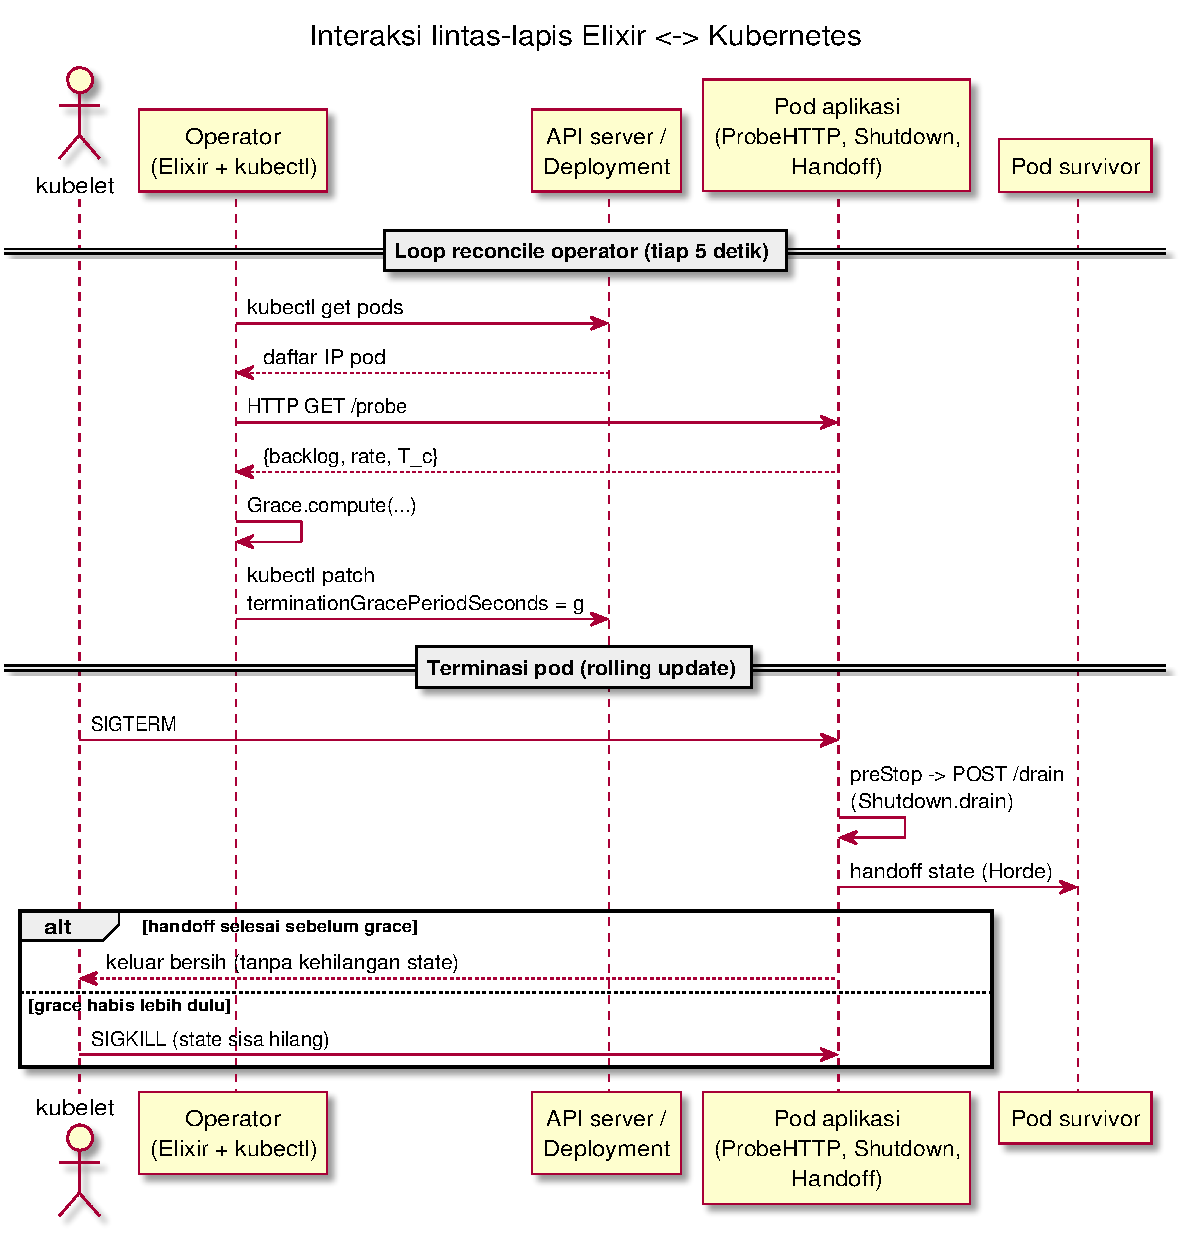
\includegraphics[width=0.82\linewidth]{fig/seq_crosslayer.pdf}
  \caption{\emph{Sequence diagram} (UML) interaksi lintas-lapis Elixir $\leftrightarrow$ Kubernetes.
  Atas: operator membaca pod (\code{kubectl get pods}), membaca \code{/probe} tiap pod, menghitung
  grace (\code{Grace.compute}), lalu menambal \code{terminationGracePeriodSeconds} Deployment. Bawah:
  \code{kubelet} mengirim \texttt{SIGTERM}, \texttt{preStop} memanggil \code{/drain}, state di-handoff
  ke pod survivor; blok \texttt{alt} menunjukkan keluar bersih vs \texttt{SIGKILL} (state hilang) bila
  grace keburu habis.}
  \label{fig:seq-crosslayer}
\end{figure}

\subsection{Alur A --- Eksperimen drain 2-node lokal (tanpa Kubernetes)}
Ini adalah cara termurah memvalidasi logika inti, dijalankan oleh \code{cluster\_probe.exs} dan
\code{harness/run.exs}. ``primary'' = node yang akan pergi; ``peer/survivor'' = node yang bertahan.

\begin{enumerate}
  \item \textbf{Bentuk cluster 2-node.} Skrip memulai sebuah node BEAM kedua di host yang sama lewat
  \code{:peer.start/1}, lalu menyalin path kode dan konfigurasi ke sana dan menjalankan aplikasi
  (\code{ensure\_all\_started}). Kedua node terhubung dan berbagi \code{Horde.Registry}.
  \item \textbf{Mulai worker di node yang akan pergi.} \code{Workers.start\_many\_local(B, ...)}
  membuat $B$ worker stateful \emph{semuanya di primary} (node yang akan dikosongkan). Ini menumpuk
  backlog $|H| = B$.
  \item \textbf{Baca probe.} \code{Probe.reading()} melaporkan backlog dan laju $\rho$ (EWMA, atau laju
  konfigurasi bila belum ada pengukuran).
  \item \textbf{Hitung grace.} Untuk policy \code{:m3}, \code{Grace.compute/2} menghitung
  $g = \mathrm{clamp}(T_d + |H|/\rho + T_c + \sigma, g_{\min}, g_{\max})$. Untuk baseline, grace tetap
  (30/300/static).
  \item \textbf{Jalankan handoff.} \code{Handoff.drain(g*1000, rate)} memindahkan worker satu-per-satu
  ke survivor: baca state $\rightarrow$ matikan lokal $\rightarrow$ hidupkan di survivor dengan state
  itu, di-throttle ke \code{rate} proses/detik.
  \item \textbf{Hasil.}
  \begin{itemize}
    \item Jika grace cukup: semua worker pindah, \code{drain} mengembalikan \code{:ok},
    \code{local\_count} primary menjadi 0 dan survivor menjadi $B$. State (mis. counter
    \code{updates}) tetap utuh --- inilah yang diuji \code{cluster\_handoff\_test.exs}.
    \item Jika grace \emph{terlalu pendek}: \code{drain} mengembalikan \code{\{:timeout, remaining\}}
    dengan \code{remaining > 0}. Worker sisa itu (dan datanya) ``hilang'' --- ini kasus kehilangan
    state RQ1.
  \end{itemize}
\end{enumerate}

\subsection{Alur B --- Loop Kubernetes nyata}
Saat dideploy di Kubernetes (manifest di \code{code/k8s/}), loop lintas-lapis berjalan terus-menerus:

\begin{enumerate}
  \item \textbf{Operator melihat daftar pod.} Tiap 5 detik, \code{Operator.reconcile/0} memanggil
  \code{kubectl get pods} (lewat \code{pod\_ips/0}) untuk mendapat IP semua pod app.
  \item \textbf{Operator membaca tiap \texttt{/probe}.} \code{probe(ip)} melakukan HTTP GET ke
  \code{http://<ip>:4000/probe} dan mem-parsing JSON menjadi \code{\%\{backlog, rate\_eps, t\_c\_ms\}}.
  \item \textbf{Operator menghitung grace.} Untuk tiap pembacaan, \code{Grace.compute/2} dipanggil;
  operator mengambil nilai \emph{terbesar} (\code{Enum.max}) agar aman bagi pod tersibuk.
  \item \textbf{Operator menambal Deployment.} \code{patch\_grace/1} menyusun patch JSON dan
  menjalankan \code{kubectl patch deployment} untuk men-set
  \code{terminationGracePeriodSeconds = grace}. Rolling update berikutnya akan memakai grace ini.
  \item \textbf{Hook \texttt{preStop} men-drain saat \texttt{SIGTERM}.} Saat Kubernetes mematikan
  sebuah pod, ia menjalankan hook \code{preStop} di \code{app.yaml} \emph{sebelum} mengirim
  \code{SIGTERM}: hook itu \code{wget} ke \code{POST /drain}. Endpoint \code{/drain} memanggil
  \code{Shutdown.drain\_and\_await()} yang \emph{memblok} sampai handoff selesai. Karena Kubernetes
  menunggu \code{preStop} selesai (dibatasi \code{terminationGracePeriodSeconds}), pod tidak mati
  sebelum handoff beres --- selama grace mencukupi.
\end{enumerate}

Bukti nyata: di cluster \code{kind} 3-replika, operator menambal grace Deployment dari 6 detik (idle)
menjadi 26 detik setelah $\sim$190 proses stateful/pod menumpuk pada laju 10/detik --- loop
lintas-lapis terkonfirmasi di orkestrator nyata.

% =============================================================================
\section{Bagaimana Kode Menjawab RQ1--RQ8}
\label{sec:rq}

Tabel berikut memetakan tiap research question ke kode dan datanya; tiap RQ dijelaskan satu paragraf
setelahnya. (Teks RQ dikutip dari \code{paper/main.tex}.)

\begin{longtable}{@{}p{0.06\linewidth} p{0.27\linewidth} p{0.28\linewidth} p{0.30\linewidth}@{}}
\toprule
\textbf{RQ} & \textbf{Fokus} & \textbf{Kode penghasil} & \textbf{Data / Figur} \\
\midrule
\endhead
RQ1 & correctness (kehilangan state) & \code{run.exs}, \code{sweep.exs}, \code{cluster\_handoff\_test.exs} & \code{results\_runs.csv}, \code{results\_sweep.csv} $\rightarrow$ \code{eval\_state\_loss.pdf}, \code{eval\_sweep\_loss.pdf}, \code{eval\_invariant.pdf} \\
RQ2 & efficiency (grace \& waktu rollout) & \code{run.exs}, \code{sweep.exs} & \code{results\_runs.csv}, \code{results\_sweep.csv}, \code{results\_rollout.csv} $\rightarrow$ \code{eval\_grace\_budget.pdf}, \code{eval\_sweep\_grace.pdf}, \code{eval\_rollout.pdf} \\
RQ3 & adaptivity (grace mengikuti beban) & \code{sweep.exs} (sweep beban) & \code{results\_sweep.csv} $\rightarrow$ \code{eval\_sweep\_grace.pdf} \\
RQ4 & overhead & \code{sweep.exs} ($\rightarrow$ \code{Harness.overhead/1}) & \code{results\_overhead.csv} \\
RQ5 & robustness (sensitivitas) & \code{sweep.exs} (bagian D) & \code{results\_sensitivity.csv} $\rightarrow$ \code{eval\_sensitivity.pdf} \\
RQ6 & scalability ($|H|$ 1k..40k) & \code{scale.exs} ($\rightarrow$ \code{Harness.scale/1}) & \code{results\_scale.csv} $\rightarrow$ \code{eval\_scale.pdf} \\
RQ7 & network realism (latensi nyata) & \code{k8s/netem.sh} (tc netem di kind) & \code{results\_netem.csv} $\rightarrow$ \code{eval\_netem.pdf} \\
RQ8 & realistic workload (Phoenix.Presence) & \code{presence.exs} (\code{Phoenix.Tracker}) & \code{results\_presence.csv} $\rightarrow$ \code{eval\_presence.pdf} \\
\bottomrule
\end{longtable}

\paragraph{RQ1 (correctness).} ``Apakah grace tetap kehilangan state saat handoff melebihi grace, dan
apakah controller menghilangkan kehilangan itu?'' \code{cluster\_handoff\_test.exs} membuktikan dua
arah pada cluster 2-node nyata: grace longgar $\rightarrow$ \code{:ok}, state utuh; grace terlalu
pendek $\rightarrow$ \code{\{:timeout, remaining>0\}}. Pada data: grace tetap 30 detik kehilangan
40 dari 160 proses begitu kebutuhan $>$ grace, sedangkan adaptif kehilangan 0.

\paragraph{RQ2 (efficiency).} ``Seberapa banyak grace yang diberikan controller dibanding grace tetap
berlebih, dan bagaimana tiap policy memengaruhi waktu rolling-update?'' Adaptif memilih grace 16--46
detik sesuai kebutuhan, dibanding tetap 300 detik yang $\sim$6--7$\times$ berlebih.
\code{eval\_rollout.pdf} membandingkan waktu rollout 3-pod antar policy.

\paragraph{RQ3 (adaptivity).} ``Apakah grace yang diberikan mengikuti beban?'' \code{run\_sweep/3}
menyapu kebutuhan handoff \{10, 25, 40\} detik; kurva grace adaptif naik mengikuti kebutuhan
(\code{eval\_sweep\_grace.pdf}), sementara baseline tetap datar (dan baseline pendek mulai kehilangan
state saat kebutuhan melewatinya).

\paragraph{RQ4 (overhead).} ``Berapa biaya controller (latensi probe, memori per-proses, throughput
handoff, jejak operator)?'' \code{Harness.overhead/1} mengukur ketiganya. Hasil tercatat: probe
$\sim$7 µs, $\sim$6{,}7 KB/proses, $\sim$8{,}3k handoff/detik; operator di kind $\sim$73 MiB dan
$\sim$74 ms reconcile/5 detik.

\paragraph{RQ5 (robustness).} ``Seberapa sensitif grace terhadap margin, batas, dan galat estimasi
laju?'' Bagian D di \code{sweep.exs} memvariasikan $\sigma \in \{0,5,10,15\}$, $g_{\max} \in \{30,60,
120,300\}$, dan faktor galat laju $\{0{,}5; 1{,}0; 2{,}0\}$, menghasilkan \code{eval\_sensitivity.pdf}.

\paragraph{RQ6 (scalability).} ``Bagaimana biaya drain satu node menskala dengan backlog $|H|$, dan di
mana plafon per-node?'' \code{scale.exs} menyapu $|H| = 1\text{k} \rightarrow 40\text{k}$. Memori naik
linear dan murah ($\sim$4 KB/proc), tetapi throughput handoff \emph{ambruk super-linear}
(3003 $\rightarrow$ 67 proc/detik) saat registry delta-CRDT terisi. Plafon per-node di $|H|=40$k: node
tidak selesai drain dalam 600 detik $\rightarrow$ 19.392/40.000 hilang. Figur: \code{eval\_scale.pdf}.

\paragraph{RQ7 (network realism).} ``Di bawah latensi antar-pod nyata, apakah estimasi laju --- dan
karenanya grace --- mengikuti throughput handoff yang menurun?'' \code{k8s/netem.sh} menyuntik
\code{tc netem} pada egress pod survivor di kind, mengukur RTT nyata; $\rho \approx 1/\text{RTT}$
ambruk (23.810 $\rightarrow$ 6{,}7/detik), dan grace naik hingga plafon $g_{\max}$. Figur:
\code{eval\_netem.pdf}.

\paragraph{RQ8 (realistic workload).} ``Apakah mekanisme tetap berlaku pada fitur terdistribusi yang
umum dipakai (Phoenix.Presence), dan berapa $T_c$ nyata yang harus ditutup grace?'' \code{presence.exs}
melacak $N$ presence di \code{Phoenix.Tracker}, men-drain node, dan mengukur re-konvergensi nyata
$T_c \approx 1{,}5$ detik (hampir konstan terhadap $N$ 100--2000), $\sim$30$\times$ heuristik 50 ms,
namun tertutup $\sigma = 5$ detik. Figur: \code{eval\_presence.pdf}.

% =============================================================================
\section{Panduan Menjalankan Eksperimen untuk Semua RQ}
\label{sec:menjalankan}

Bagian ini memberi perintah \textbf{persis} untuk mereproduksi tiap RQ, langkah demi langkah. Kecuali
disebutkan, semua perintah BEAM dijalankan dari \code{code/app}.

\paragraph{Persiapan satu kali (semua RQ lokal).}
Persiapan satu kali (semua RQ lokal).

\begin{lstlisting}[style=sh]
cd code/app
mix deps.get        # unduh dependency (Horde, libcluster, Bandit, Plug, Jason, phoenix_pubsub)
mix compile         # kompilasi
mix test            # 6 unit test Grace (suite :cluster dikecualikan secara default)
\end{lstlisting}

\paragraph{Singkatan peluncur node terdistribusi.} Hampir semua harness butuh ``primary''
terdistribusi (ia memunculkan peer survivor sendiri). Pola peluncurannya:
\begin{lstlisting}[style=sh]
# Pola umum (dijalankan dari code/app):
MIX_ENV=test elixir --name primary@127.0.0.1 --cookie ck -S mix run harness/<skrip>.exs
\end{lstlisting}

\begin{quote}
\textbf{PERINGATAN KERAS.} \emph{Jangan pernah} menjalankan
\code{pkill -f '...@127.0.0.1'} untuk membersihkan beam: pola itu juga cocok dengan baris perintah
shell yang sedang berjalan, sehingga \textbf{mematikan shell Anda sendiri} (keluar dengan kode 144,
tanpa output). Matikan beam yatim berdasarkan \textbf{PID} saja.
\end{quote}

\subsection{RQ1 \& RQ2 --- correctness \& efficiency (tabel dua beban)}
\begin{lstlisting}[style=sh]
cd code/app
# (opsional) validasi logika inti pada cluster 2-node nyata:
MIX_ENV=test elixir --name primary@127.0.0.1 --cookie ck -S mix test --only cluster
# tabel dua beban -> data/results_runs.csv :
MIX_ENV=test elixir --name primary@127.0.0.1 --cookie ck -S mix run harness/run.exs
# render figur:
~/venv/bin/python ../analysis/plot.py
\end{lstlisting}
Menghasilkan \code{eval\_state\_loss.pdf} dan \code{eval\_grace\_budget.pdf} (juga
\code{eval\_invariant.pdf} bila \code{results\_sweep.csv} sudah ada).

\subsection{RQ2, RQ3, RQ4, RQ5 --- sweep, rollout, overhead, sensitivitas}
Keempatnya dihasilkan satu skrip:
\begin{lstlisting}[style=sh]
cd code/app
MIX_ENV=test elixir --name primary@127.0.0.1 --cookie ck -S mix run harness/sweep.exs
~/venv/bin/python ../analysis/plot.py
\end{lstlisting}
Menulis \code{results\_sweep.csv} (RQ1/RQ2/RQ3 kurva), \code{results\_rollout.csv} (RQ2),
\code{results\_overhead.csv} (RQ4), \code{results\_sensitivity.csv} (RQ5). Figur terkait:
\code{eval\_sweep\_loss.pdf}, \code{eval\_sweep\_grace.pdf}, \code{eval\_invariant.pdf},
\code{eval\_rollout.pdf}, \code{eval\_sensitivity.pdf}.

\subsection{Statistik (confidence interval) --- pengulangan}
\begin{lstlisting}[style=sh]
cd code/app
MIX_ENV=test elixir --name primary@127.0.0.1 --cookie ck -S mix run harness/repeats.exs
\end{lstlisting}
Menulis \code{results\_runs\_ci.csv} (tabel beban $\times$ 4 policy $\times$ 10 ulang) dan
\code{results\_rollout\_ci.csv} (rollout $\times$ 4 policy $\times$ 5 ulang). Loss/grace persis
ter-reproduksi (CI=0); drain $\pm$0{,}003 detik (CI95).

\subsection{RQ6 --- scalability ($|H|$ 1k..40k)}
\begin{lstlisting}[style=sh]
cd code/app
MIX_ENV=test elixir --name primary@127.0.0.1 --cookie ck -S mix run harness/scale.exs
~/venv/bin/python ../analysis/plot.py
\end{lstlisting}
Menulis \code{results\_scale.csv} (streaming tiap ukuran) dan figur \code{eval\_scale.pdf}. Skrip
berhenti otomatis jika start cost atau memori membatasi.

\subsection{RQ8 --- realistic workload (Phoenix.Presence)}
\begin{lstlisting}[style=sh]
cd code/app
MIX_ENV=test elixir --name primary@127.0.0.1 --cookie ck -S mix run harness/presence.exs
~/venv/bin/python ../analysis/plot.py
\end{lstlisting}
Menulis \code{results\_presence.csv} dan figur \code{eval\_presence.pdf}.

\subsection{RQ7 \& Kubernetes --- latensi nyata + fail-safe}
RQ7 dan validasi fail-safe berjalan di cluster \code{kind} sungguhan. Pertama, siapkan cluster:
\begin{lstlisting}[style=sh]
# dari root proyek 01_cross_layer_grace_controller/
kind create cluster --name grace
docker build -t grace:dev code/                 # bangun image (konteks build = code/)
kind load docker-image grace:dev --name grace
kubectl apply -f code/k8s/rbac.yaml -f code/k8s/app.yaml -f code/k8s/operator.yaml
kubectl rollout status deploy/grace
kubectl logs deploy/grace-operator              # "operator: pods=N grace=Ms"
\end{lstlisting}
Lalu jalankan eksperimen:
\begin{lstlisting}[style=sh]
bash code/k8s/netem.sh      # RQ7: latensi nyata -> RTT, rho, grace -> data/results_netem.csv
bash code/k8s/faults.sh     # fail-safe: crash operator / probe rusak / RBAC dicabut
~/venv/bin/python code/analysis/plot.py   # render eval_netem.pdf
kind delete cluster --name grace           # bersihkan
\end{lstlisting}

\begin{quote}
\textbf{PERINGATAN RQ7 (netem).} Untuk \code{netem.sh}, \emph{matikan/scale operator dulu}
(\code{kubectl scale deploy/grace-operator --replicas=0}) --- kalau tidak, backlog yang dibuat
eksperimen membuat operator menambal grace, memicu rolling update yang mematikan pod ``leaver'' di
tengah pengukuran (keluar 137). Skrip \code{netem.sh} sudah melakukan ini otomatis dan memulihkannya
saat keluar. Selain itu, injeksi latensi diberikan pada \emph{egress survivor}, bukan pada leaver
(memperlambat leaver akan memutus koneksi distribusi helper \code{rpc}).
\end{quote}

% =============================================================================
\section{\texorpdfstring{Tabel Pemetaan Ringkas (RQ $\rightarrow$ Skrip $\rightarrow$ CSV $\rightarrow$ Figur)}{Tabel Pemetaan Ringkas (RQ - Skrip - CSV - Figur)}}
\label{sec:pemetaan}

\begin{longtable}{@{}p{0.06\linewidth} p{0.24\linewidth} p{0.34\linewidth} p{0.27\linewidth}@{}}
\toprule
\textbf{RQ} & \textbf{Skrip harness} & \textbf{File CSV} & \textbf{File figur (PDF)} \\
\midrule
\endhead
RQ1 & \code{run.exs}, \code{sweep.exs} & \code{results\_runs.csv}, \code{results\_sweep.csv} & \code{eval\_state\_loss.pdf}, \code{eval\_sweep\_loss.pdf}, \code{eval\_invariant.pdf} \\
RQ2 & \code{run.exs}, \code{sweep.exs} & \code{results\_runs.csv}, \code{results\_sweep.csv}, \code{results\_rollout.csv} & \code{eval\_grace\_budget.pdf}, \code{eval\_sweep\_grace.pdf}, \code{eval\_rollout.pdf} \\
RQ3 & \code{sweep.exs} & \code{results\_sweep.csv} & \code{eval\_sweep\_grace.pdf} \\
RQ4 & \code{sweep.exs} & \code{results\_overhead.csv} & (tabel di paper) \\
RQ5 & \code{sweep.exs} & \code{results\_sensitivity.csv} & \code{eval\_sensitivity.pdf} \\
RQ6 & \code{scale.exs} & \code{results\_scale.csv} & \code{eval\_scale.pdf} \\
RQ7 & \code{k8s/netem.sh} & \code{results\_netem.csv} & \code{eval\_netem.pdf} \\
RQ8 & \code{presence.exs} & \code{results\_presence.csv} & \code{eval\_presence.pdf} \\
-- & \code{repeats.exs} & \code{results\_runs\_ci.csv}, \code{results\_rollout\_ci.csv} & (statistik/CI) \\
\bottomrule
\end{longtable}

% =============================================================================
\section{Glosarium Singkat}
\label{sec:glosarium}

\begin{description}[leftmargin=1.6em,style=nextline]
  \item[SIGTERM] Sinyal sistem operasi yang artinya ``tolong berhenti dengan rapi''. Bisa ditangani
  proses untuk pembersihan. Kubernetes mengirimnya di awal terminasi pod.
  \item[SIGKILL] Sinyal yang \emph{tidak bisa} ditangkap/diabaikan; proses langsung mati. Kubernetes
  mengirimnya setelah grace period habis.
  \item[grace period] Waktu toleransi (\code{terminationGracePeriodSeconds}) antara SIGTERM dan SIGKILL
  yang diberikan untuk berberes.
  \item[rolling update] Memperbarui aplikasi secara bertahap (pod demi pod) agar layanan tetap hidup
  selama pembaruan.
  \item[pod] Unit terkecil yang dijadwalkan Kubernetes; membungkus satu container (atau beberapa) yang
  berbagi jaringan/penyimpanan.
  \item[drain] Proses \emph{mengosongkan} sebuah node/pod yang akan dimatikan dari pekerjaannya
  sebelum ia benar-benar mati: menyelesaikan permintaan yang masih berjalan, lalu mem-\emph{handoff}
  semua proses stateful-nya ke node lain. ``Satu drain'' = satu kali menjalankan proses ini
  (\code{Handoff.drain/2}): ulangi ``baca state worker $\rightarrow$ pindah ke survivor'' sampai
  backlog 0 \emph{atau} grace habis (sisa yang belum terpindah hilang). Analogi: mengosongkan satu
  kamar sebelum dibongkar.
  \item[handoff] Pemindahan state in-memory dari node yang akan mati ke node yang bertahan
  (baca $\rightarrow$ matikan lokal $\rightarrow$ hidupkan di survivor). Satu drain terdiri dari banyak
  handoff (satu per worker).
  \item[CRDT] \emph{Conflict-free Replicated Data Type}: struktur data yang bisa diubah di banyak node
  dan otomatis merge ke hasil sama tanpa koordinasi pusat.
  \item[GenServer] ``Server process'' OTP dengan state privat yang menangani pesan satu per satu
  (lewat \code{call} sinkron atau \code{cast} asinkron).
  \item[supervisor] Proses pengawas yang menjalankan dan me-restart proses anak bila mati
  (``let it crash''). \code{DynamicSupervisor} = anak dibuat sesuai kebutuhan saat runtime.
  \item[EWMA] \emph{Exponentially Weighted Moving Average}: rata-rata berjalan yang memberi bobot lebih
  besar pada sampel terbaru. Dipakai Probe untuk menaksir laju handoff $\rho$.
  \item[RPC] \emph{Remote Procedure Call}: menjalankan fungsi di node lain dan mengembalikan hasilnya
  (di Erlang/Elixir lewat \code{:rpc.call/4}).
  \item[PID] \emph{Process IDentifier}: pengenal sebuah proses BEAM. Worker dialamatkan lewat via-tuple
  Horde, bukan PID mentah, agar tetap valid setelah pindah node.
  \item[libcluster] Library yang membentuk cluster BEAM otomatis (strategi Gossip lokal, strategi
  Kubernetes di cluster).
  \item[Horde] Library registry/supervisor terdistribusi berbasis delta-CRDT; di sini memberi identitas
  unik se-cluster bagi tiap worker.
  \item[operator] Program yang terus mengawasi dan mendamaikan kondisi cluster ke kondisi yang
  diinginkan. Di sini: membaca probe lalu menambal grace.
  \item[PodDisruptionBudget (PDB)] Aturan Kubernetes yang membatasi berapa banyak pod boleh tidak
  tersedia sekaligus saat gangguan sukarela (mis. drain node), menjaga ketersediaan minimum.
  \item[$T_c$ (waktu konvergensi)] Waktu agar cluster ``tenang'' kembali (membership stabil, registry
  sinkron) setelah node pergi.
  \item[$T_d$ (waktu drain)] Waktu menyelesaikan permintaan yang sedang berjalan sebelum state
  dipindahkan.
  \item[$\rho$ (laju handoff)] Berapa proses per detik yang bisa dipindahkan (ditaksir Probe via EWMA).
  \item[$|H|$ (backlog)] Jumlah proses stateful yang masih harus dipindahkan dari node yang akan pergi.
  \item[$\sigma$ (margin keamanan)] Detik tambahan pada estimasi grace agar tidak pas di tepi.
\end{description}

\bigskip
\hrule
\medskip
\noindent\emph{Catatan akurasi: seluruh nama fungsi, file, perintah, dan angka dalam dokumen ini
diambil langsung dari kode sumber dan dokumentasi di
\code{01\_cross\_layer\_grace\_controller/}. Bila ada perbedaan kecil antara paper dan kode
(mis. peran ``operator'' di paper disebut Bonny, sedangkan kode memakai operator berbasis
\code{kubectl}), dokumen ini mengikuti \emph{kode} sebagai sumber kebenaran.}

\end{document}
